%%-*-latex-*-

\documentclass[wide]{slides}

% Language
%
\usepackage{hyphenat}          % \hyp{} is a breakable dash
\usepackage{alltt}
\usepackage{xspace}

\frenchspacing  % Follow French conventions after a period

% Graphics
%
\usepackage{graphicx}

% Maths & Logic
%
\usepackage{amsmath,amssymb,amsthm,stmaryrd}
\usepackage{mathpartir}

% New commands
%
% PascaLIGO

\newcommand{\Kand}[0]{\textbf{and}\xspace}
\newcommand{\Kattributes}[0]{\textbf{attributes}\xspace}
\newcommand{\Kbegin}[0]{\textbf{begin}\xspace}
\newcommand{\Kbigmap}[0]{\textbf{big_map}\xspace}
\newcommand{\Kblock}[0]{\textbf{block}\xspace}
\newcommand{\Kcase}[0]{\textbf{case}\xspace}
\newcommand{\Kconst}[0]{\textbf{const}\xspace}
\newcommand{\Kcontains}[0]{\textbf{contains}\xspace}
\newcommand{\Kelse}[0]{\textbf{else}\xspace}
\newcommand{\Kend}[0]{\textbf{end}\xspace}
\newcommand{\KFalse}[0]{\textbf{False}\xspace}
\newcommand{\Kfor}[0]{\textbf{for}\xspace}
\newcommand{\Kfrom}[0]{\textbf{from}\xspace}
\newcommand{\Kfunction}[0]{\textbf{function}\xspace}
\newcommand{\Kif}[0]{\textbf{if}\xspace}
\newcommand{\Kin}[0]{\textbf{in}\xspace}
\newcommand{\Kis}[0]{\textbf{is}\xspace}
\newcommand{\Klist}[0]{\textbf{list}\xspace}
\newcommand{\Kmap}[0]{\textbf{map}\xspace}
\newcommand{\Kmod}[0]{\textbf{mod}\xspace}
\newcommand{\Knil}[0]{\textbf{nil}\xspace}
\newcommand{\Knot}[0]{\textbf{not}\xspace}
\newcommand{\Kof}[0]{\textbf{of}\xspace}
\newcommand{\Kor}[0]{\textbf{or}\xspace}
\newcommand{\Kpatch}[0]{\textbf{patch}\xspace}
\newcommand{\Krecord}[0]{\textbf{record}\xspace}
\newcommand{\Kremove}[0]{\textbf{remove}\xspace}
\newcommand{\Kset}[0]{\textbf{set}\xspace}
\newcommand{\Kskip}[0]{\textbf{skip}\xspace}
\newcommand{\Kthen}[0]{\textbf{then}\xspace}
\newcommand{\Kto}[0]{\textbf{to}\xspace}
\newcommand{\KTrue}[0]{\textbf{True}\xspace}
\newcommand{\Ktype}[0]{\textbf{type}\xspace}
\newcommand{\KUnit}[0]{\textbf{Unit}\xspace}
\newcommand{\Kvar}[0]{\textbf{var}\xspace}
\newcommand{\Kwhile}[0]{\textbf{while}\xspace}
\newcommand{\Kwith}[0]{\textbf{with}\xspace}

% CameLIGO
%
% Begin
% Else
% End
\newcommand{\Kfalse}[0]{\textbf{false}\xspace}
\newcommand{\Kfun}[0]{\textbf{fun}\xspace}
% If
% In
\newcommand{\Klet}[0]{\textbf{let}\xspace}
\newcommand{\Kmatch}[0]{\textbf{match}\xspace}
% Mod
% Not
% Of
% Or
% Then
\newcommand{\Ktrue}[0]{\textbf{true}\xspace}
% Type
% With

% ReasonLIGO
%
% Else
% False
% If
% Let
\newcommand{\Kswitch}[0]{\textbf{switch}\xspace}
% Mod
% Or
% True
% Type

% Comments
\newcommand{\com}[1]{\textcolor{blue}{{#1}}}

% ----------------------------------------------------------------
% Document
%

\maintitle{Smart Contracts in LIGO}
\mainauthor{\textbf{Christian Rinderknecht}\\
  {\small\url{rinderknecht@free.fr}}\\
Ligo LANG}
\confname{Tezos Developers Day}
\confshortname{Tezos}
\confdate{6 March 2020}

\begin{document}

\maketitle

%% \begin{slide}
%%   \title{A personal introduction}

%%   \begin{itemize}

%%     \item My alma mater is \emph{Universit\'e Pierre et Marie Curie}
%%       (UPMC, a.k.a. Paris~6).

%%     \item My PhD advisor was Michel Mauny, at INRIA, one of the most
%%       prestigious research institutes in informatics in France.

%%     \item I was a member of the team that developed the programming
%%       language OCaml.

%%     \item I went on to work as an engineer, a researcher and a
%%       professor for many years, across several countries (France,
%%       Korea, Hungary, Sweden), both in academia and private
%%       companies.

%%     \item In \oldstylenums{2018}, I joined Nomadic Labs, where a lot
%%       of the maintenance of the Tezos blockchain is done. My expertise
%%       is in compiler construction and functional programming. I have
%%       been working on a high-level language for writing smart
%%       contracts on Tezos.

%%   \end{itemize}

%% \end{slide}


%% \begin{slide}
%%   \title{A personal introduction}

%%   \begin{minipage}{0.5\linewidth}
%%     My book about functional programming is published in London!
%%   \end{minipage}%
%%   \begin{minipage}{0.5\linewidth}
%%     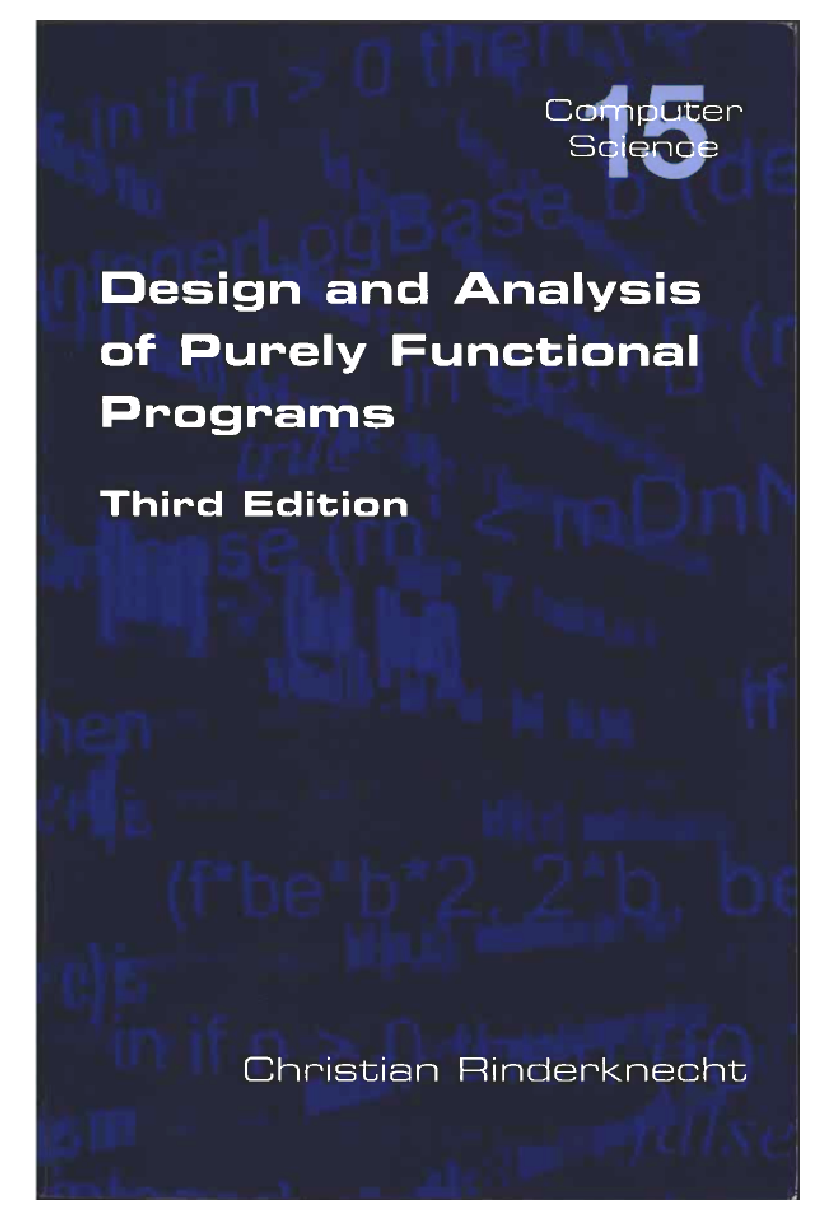
\includegraphics[scale=0.35]{my_book.eps}
%%   \end{minipage}%

%% \end{slide}

\begin{slide}
  \title{LIGO}

  \begin{itemize}

    \item I joined Nomadic Labs in July 2018.

    \item Two of my colleagues were Suzanne Dupéron and Gabriel
      Alfour.

    \item Mi-2019, Gabriel founded \textbf{Ligo LANG}, a spin-off
      company and Suzanne and I joined him.

    \item Ligo LANG is funded by the Tezos Foundation to develop tools
      to ease the creation of distributed applications on Tezos.

    \item We are currently a small group of engineers located around
      the globe. (Matej \v{S}ima of Stove Labs worked with us and is
      still close.)

    \item We have designed a language for smart contract on Tezos,
      called \textbf{LIGO}.

    \item We have written a compiler from LIGO to Michelson.

  \end{itemize}

\end{slide}

\begin{slide}
  \title{Tooling for LIGO}

  \begin{itemize}

    \item Several tools have been developed, aiming at facilitating
      the adoption of LIGO.

    \item \textbf{A VSCode plug-in} is available,
      featuring
      \begin{itemize}

        \item syntax highlighting,

        \item one-click compilation to Michelson,

        \item \emph{dry runs} to locally execute contracts on a
          sandbox.

%        \item a reactive counter estimating the gas consumption.

      \end{itemize}

    \item The architecture of VSCode, with its Language Server
      Protocol, hopefully opens the door to plugins written in any
      programming language, e.g., static analysis in OCaml.

    \item \textbf{A web-based IDE} with the same set of features:\\
      \url{https://ide.ligolang.org/}

%    \item Start here: \url{https://ligolang.org/}

  \end{itemize}

\end{slide}

\begin{slide}
  \title{LIGO}

  \begin{itemize}

    \item Ligo LANG also helps with the training of Tezos users.

    \item Unlike Michelson, LIGO is a language akin to what a
      mainstream programmer would expect.

    \item This means that LIGO features variables, expressions,
      function calls, data types, pattern matching etc.

    \item Nevertheless, LIGO is a Domain Specific Language (DSL) for
      Tezos.

    \item It is an \textbf{open source, collective project} (under the
      MIT licence).

    \item It is hosted here: \url{https://ligolang.org/}

    \item Anyone can register an issue with our gitlab server:\\
      \url{https://gitlab.com/ligolang/ligo/}

  \end{itemize}

\end{slide}

\begin{slide}
  \title{LIGO}

  \begin{itemize}

    \item We are asked sometimes to compare LIGO with other languages.

    \item This is difficult because we do not know well enough the
      other languages.
      \begin{center}
        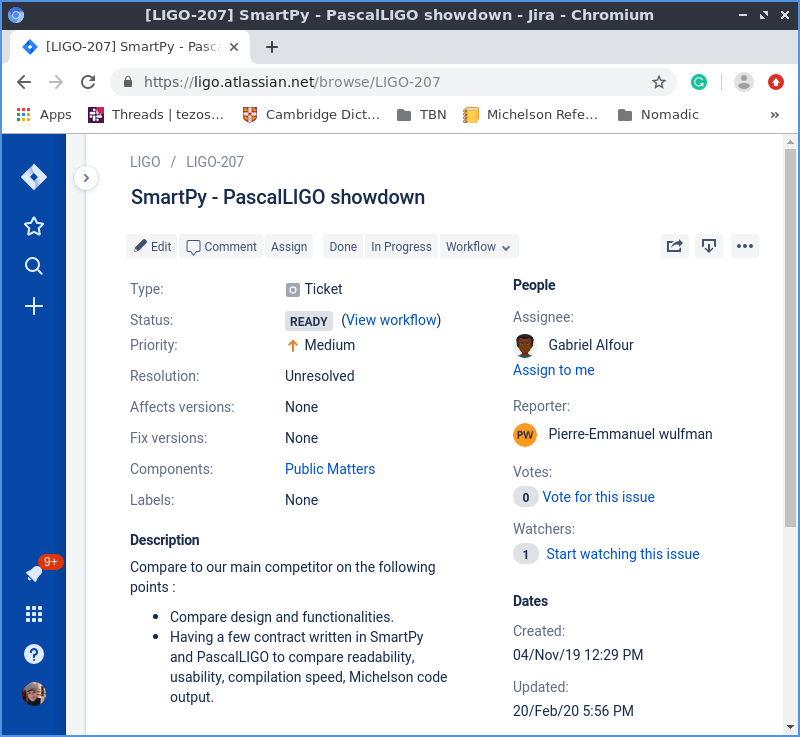
\includegraphics[scale=0.3]{ligo_smartpy.png}
      \end{center}

  \end{itemize}

\end{slide}

\begin{slide}
  \title{LIGO is polyglot}

  \begin{itemize}

    \item Perhaps the most striking feature of LIGO is that it comes
      in \textbf{different concrete syntaxes}, and even
      \textbf{different programming paradigms}.

    \item In other words, LIGO is not defined by one syntax and one
      paradigm, like imperative versus functional.

    \item There is \textbf{PascaLIGO}, which is inspired by Pascal,
      hence is an imperative language with lots of keywords, where
      values can be locally mutated from within the scope where they
      have been declared.

    \item There is \textbf{CameLIGO}, which is inspired by the pure
      subset of OCaml, hence is a functional language with few
      keywords, where values cannot be mutated, but still require type
      annotations (unlike OCaml, whose compiler performs almost full
      type inference).

    \item There is \textbf{ReasonLIGO}, which is inspired by the pure
      subset of ReasonML, which is a JavaScript syntax on top of
      OCaml.

  \end{itemize}

\end{slide}

\begin{slide}
  \title{LIGO is polyglot}

  \begin{itemize}

    \item Even within PascaLIGO, two styles are possible: terse or
      verbose. We illustrate the terse style here and in the
      documentation. We plan to offer automatic style checking and
      two-way conversion by \textbf{pretty\hyp{}printing}.

    \item We plan to provide \textbf{transpilation between syntaxes},
      which includes pretty-printing. Two reasons:
      \begin{enumerate}

        \item Some large owners of contracts may not want to depend
          too much on the given skill set of their maintainers.

        \item The more reviewed a smart contract is, the better,
          therefore it is beneficial to present one contract in the
          syntax that is better understood by a reviewer.

      \end{enumerate}

  \end{itemize}

\end{slide}


\begin{slide}
  \title{Some non-Tezos-specific LIGO features}

  \begin{itemize}

    \item At the call site of a function, \textbf{the arguments and
      the environment are copied}, therefore any mutation (in
      PascaLIGO) will have no effect on the caller's arguments or the
      environment at the call site.

    \item LIGO features \textbf{higher-order functions}, that is,
      functions can be passed as arguments to others.

    \item There are \textbf{no user-defined recursive data types}
      (only predefined, like lists, sets and maps).

    \item Currently, there are no user-defined recursive functions,
      but we are going to enable very soon \textbf{tail recursive
        functions}.

  \end{itemize}

\end{slide}

\begin{slide}
  \title{Variant Types}

  \begin{itemize}

    \item A variant type is a user-defined or a built-in type (in case
      of options) that defines a type by cases, so a value of a
      variant type is either this, or that or... and nothing else. The
      simplest variant type is equivalent to the enumerated types
      found in Java.

    \item In PascaLIGO:
      \begin{alltt}
\Ktype coin \Kis Head | Tail
\Kconst head : coin = Head \com{// Equivalent to Head (Unit)}
\Kconst tail : coin = Tail \com{// Equivalent to Tail (Unit)}
      \end{alltt}

      \vspace{-5mm}
    \item In CameLIGO:
      \begin{alltt}
\Ktype coin = Head | Tail
\Klet head : coin = Head
\Klet tail : coin = Tail
      \end{alltt}

      \vspace{-5mm}
    \item In ReasonLIGO:
      \begin{alltt}
\Ktype coin = Head | Tail;
\Klet head : coin = Head;
\Klet tail : coin = Tail;
      \end{alltt}

  \end{itemize}

\end{slide}

\begin{slide}
  \title{Variant Types}

  \begin{itemize}

    \item A variant type is a user-defined or a built-in type (in case
      of options) that defines a type by cases, so a value of a
      variant type is either this, or that or... and nothing else. The
      simplest variant type is equivalent to the enumerated types
      found in Java.

    \item In PascaLIGO:
      \begin{alltt}
\Ktype coin \Kis Head | Tail
\Kconst head : coin = Head \com{// Equivalent to Head (Unit)}
\Kconst tail : coin = Tail \com{// Equivalent to Tail (Unit)}
      \end{alltt}

      \vspace{-5mm}
    \item In CameLIGO:
      \begin{alltt}
\Ktype coin = Head | Tail
\Klet head : coin = Head
\Klet tail : coin = Tail
      \end{alltt}

      \vspace{-5mm}
    \item In ReasonLIGO:
      \begin{alltt}
\Ktype coin = Head | Tail;
\Klet head : coin = Head;
\Klet tail : coin = Tail;
      \end{alltt}

  \end{itemize}

\end{slide}

\begin{slide}
  \title{Variant Types}

  \begin{itemize}

    \item The names \texttt{Head} and \texttt{Tail} in the definition
      of the type \texttt{coin} are called \textbf{data constructors},
      or \textbf{variants}.

    \item In general, it is interesting for variants to carry some
      information, and thus go beyond enumerated types.

    \item In the following, we show how to define different kinds of
      users of a system.

  \end{itemize}

\end{slide}

\begin{slide}
  \title{Variants in PascaLIGO}

\begin{alltt}
\Ktype id \Kis nat

\Ktype user \Kis
  Admin   \Kof id
| Manager \Kof id
| Guest

\Kconst u : user = Admin (1000n)
\Kconst g : user = Guest         \com{// Equivalent to Guest (Unit)}
\end{alltt}

\end{slide}

\begin{slide}
  \title{Variants in CameLIGO}

\begin{alltt}
\Ktype id = nat

\Ktype user =
  Admin   \Kof id
| Manager \Kof id
| Guest

\Klet u : user = Admin 1000n
\Klet g : user = Guest
\end{alltt}

\end{slide}

\begin{slide}
  \title{Variants in ReasonLIGO}

\begin{alltt}
\Ktype id = nat;

\Ktype user =
| Admin   (id)
| Manager (id)
| Guest;

\Klet u : user = Admin (1000n);
\Klet g : user = Guest;
\end{alltt}

\end{slide}

\begin{slide}
  \title{Pattern Matching}

  \begin{itemize}

    \item \textbf{Pattern matching} is similiar to the switch
      construct in Javascript, and can be used to route the program's
      control flow based on the value of a variant. Consider for
      example the definition of a function \texttt{flip} that flips a
      coin.

    \item In PascaLIGO:
      \begin{alltt}
\Ktype coin \Kis Head | Tail

\Kfunction flip (\Kconst c : coin) : coin \Kis
  \Kcase c \Kof
    Head -> Tail
  | Tail -> Head
  \Kend
      \end{alltt}

  \end{itemize}

\end{slide}

\begin{slide}
  \title{Pattern Matching in CameLIGO and ReasonLIGO}

  \begin{itemize}

    \item In CameLIGO:
      \begin{alltt}
\Ktype coin = Head | Tail

\Klet flip (c : coin) : coin =
  \Kmatch c \Kwith
    Head -> Tail
  | Tail -> Head
      \end{alltt}

    \item In ReasonLIGO:
      \begin{alltt}
\Ktype coin = Head | Tail;

\Klet flip = (c : coin) : coin =>
  \Kswitch (c) \{
  | Head => Tail
  | Tail => Head
  \};
      \end{alltt}

  \end{itemize}

\end{slide}

\begin{slide}
  \title{General Iteration in PascaLIGO}

  \begin{itemize}

    \item General iteration in PascaLIGO takes the shape of general
      loops, which should be familiar to programmers of imperative
      languages as \textbf{while loops}.

    \item Those loops are of the form
      \begin{center}
        \texttt{\textbf{while} <condition> <block>}
      \end{center}

    \item Their associated block is repeatedly evaluated until the
      condition becomes true, or never evaluated if the condition is
      false at the start. The loop never terminates if the condition
      never becomes true.

    \item Because we are writing smart contracts on Tezos, when the
      condition of a \texttt{while} loops fails to become true, the
      execution will run out of gas and stop with a failure anyway.

    \item Loops make sense only in PascaLIGO because the conditional
      expression needs to be mutated by the body of the loop.

  \end{itemize}

\end{slide}

\begin{slide}
  \title{General Iteration in PascaLIGO}

  \begin{itemize}

    \item Here is how to compute the greatest common divisors of two
      natural numbers by means of Euclid's algorithm:
      \begin{alltt}
\Kfunction gcd (\Kvar x : nat; \Kvar y : nat) : nat \Kis \Kblock \{
  \Kif x < y \Kthen \{
    \Kconst z : nat = x;
    x := y; y := z
  \}
  \Kelse \Kskip;
  \Kvar r : nat := 0n;
  \Kwhile y =/= 0n \Kblock \{
    r := x \Kmod y;
    x := y;
    y := r
  \}
\} \Kwith x
      \end{alltt}

  \end{itemize}

\end{slide}

\begin{slide}
  \title{General Iteration in CameLIGO}

  \begin{itemize}

    \item CameLIGO is a functional language where user-defined values
      are constant, therefore it makes no sense in CameLIGO to feature
      loops, which we understand as syntactic constructs where the
      state of a stopping condition is mutated, as with \texttt{while}
      loops in PascaLIGO.

    \item Instead, CameLIGO implements a \textbf{folded operation} by
      means of a predefined function named \texttt{Loop.fold\_while}.

    \item It takes an initial value of a certain type, called an
      \textbf{accumulator}, and repeatedly calls a given function,
      called \textbf{folded function}, that takes that accumulator
      and returns the next value of the accumulator, until a condition
      is met and the fold stops with the final value of the
      accumulator.

    \item The iterated function needs to have a special type: if the
      type of the accumulator is \texttt{t}, then it must have the
      type \texttt{(bool * t)} (not simply \texttt{t}). It is the
      boolean value that denotes whether the stopping condition has
      been reached.

  \end{itemize}

\end{slide}

\begin{slide}
  \title{General Iteration in CameLIGO}

  \begin{itemize}

    \item Here is how to compute the greatest common divisors of two
      natural numbers by means of Euclid's algorithm:
    \begin{alltt}
\Klet iter (x,y : nat * nat) : bool * (nat * nat) =
  \Kif y = 0n \Kthen \Kfalse, (x,y) \Kelse \Ktrue, (y, x \Kmod y)

\Klet gcd (x,y : nat * nat) : nat =
  \Klet x,y = \Kif x < y \Kthen y,x \Kelse x,y in
  \Klet x,y = Loop.fold\_while iter (x,y)
  \Kin x
    \end{alltt}

  \end{itemize}

\end{slide}

\begin{slide}
  \title{General Iteration in CameLIGO}

  \begin{itemize}

    \item To ease the writing and reading of the iterated functions
      (here, \texttt{iter}), two predefined functions are provided:
      \texttt{Loop.continue} and \texttt{Loop.stop}:
      \begin{alltt}
\Klet iter (x,y : nat * nat) : bool * (nat * nat) =
  \Kif y = 0n \Kthen Loop.stop (x,y) \Kelse Loop.resume (y, x \Kmod y)

\Klet gcd (x,y : nat * nat) : nat =
  \Klet x,y = \Kif x < y \Kthen y,x \Kelse x,y in
  \Klet x,y = Loop.fold\_while iter (x,y)
  \Kin x
      \end{alltt}

  \end{itemize}

\end{slide}

\begin{slide}
  \title{Inlining}

  \begin{itemize}

    \item The Michelson generator of the LIGO compiler performs
      several kinds of optimisations.

    \item One of them is \textbf{inlining}, that is, the expansion of
      the body of a function at its call site (with its parameters
      also expanded with the arguments).

    \item Inlining is controlled by \textbf{attributes} of constant
      and function declarations.

    \item In PascaLIGO:
      \begin{alltt}
\Kfunction fst (\Kconst p : nat * nat) : nat \Kis p.0;
\Kattributes ["inline"];

\Kfunction main (\Kconst p : nat * nat; \Kconst s : nat * nat)
  : list (operation) * (nat * nat) \Kis
  ((\Knil : list (operation)), (fst (p.0,p.1), fst (p.1,p.0)))
      \end{alltt}

  \end{itemize}

\end{slide}

\begin{slide}
  \title{Research \& Development}

  \begin{itemize}

    \item We are working on a more \textbf{powerful type system} which
      will enable the writing of more expressive contracts, featuring
      more type inference (less annotations) and enabling a greater
      variety of programming paradigms (e.g., object-oriented).

    \item We are writing a \textbf{certified backend in Coq}, that is,
      a Michelson code generator proven correct w.r.t. a formal
      semantics and extracted to OCaml.

    \item Those endeavours are not just engineering, they are
      instances of \textbf{applied research} and require a strong
      background on programming language theory.

  \end{itemize}

\end{slide}

\begin{slide}
  \title{Structure of a LIGO contract}

  \begin{itemize}

    \item A LIGO contract is a series of constant and function
      declarations.

    \item The scope of those is called \textbf{top-level}, to
      distinguish declarations that may occur within functions.

    \item In particular, even in PascaLIGO, you cannot have mutable
      variables at the top-level.

    \item As a design pattern, there is usually one special function,
      which we call \textbf{main function} that is called with a
      parameter when the contract is invoked.

    \item The main function calls other functions according to the
      value of the contract parameter.

    \item Those functions are called \textbf{entrypoints}, following
      the Michelson convention.

  \end{itemize}

\end{slide}

\end{document}
